\section{Durchführung}
\label{sec:Durchführung}

Der versuch wird nach der Abbildung \ref{fig:Aufbau} aufgebaut.
\begin{figure}[H]
    \centering
    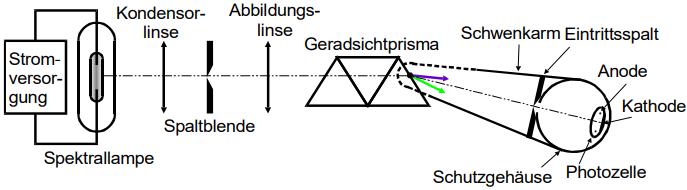
\includegraphics[scale=0.5]{content/Aufbau.png}
    \caption{Versuchsaufbau.\cite{sample}}
    \label{fig:Aufbau}
\end{figure}
Als Spektrallampe wird eine Quecksilberlampe verwendet.
Damit die Energie der Elektronen gemessen werden kann, wird ein Gegenfeld angelegt.
Durch das Geradsichtprisma lassen sich die Spektrallinien der Lampe räumlic voneinander erkennen.
Zunächst wird die Abildungslinse so verschoben, dass die Spektrallinien der Lampe scharf zu erkennen sind.
Die Photozelle wird mit dem Schwenkarm so ausgerichtet, dass eine Spektrallinie auf den Eintrittsspalt der Zelle fällt.
Die Gegenspannung wird nun zwischen $\pm \qty{2}{V}$ in $\qty{0.1}{V}$ Schritten varriert und der dazugehörige Photostrom $I_\text{ph}$ vom Picoamperemeter abgelesen. 
Diese Messung wird für drei verschiedene Spektrallinien durchgeführt.
Für die gelbe Spektrallinie wird die Messung in einem Spannungsberich von $\pm \qty{20}{V}$ gemessen.
Wenn der Photostrom sich auf $\qty{0}{A}$ annährt, wird für eine genauere Messung die Spannung un $\qty{0.05}{V}$ Schritten varriert.